
%\begin{name}
%	{Thế Nghiêm}{Sở GD \& ĐT Tỉnh Đồng Tháp}
%\end{name}
\cautl
\begin{ex}%[2D4H1-3]
	Cho hàm số $f(x) = \left( \sin \dfrac{x}{2} - \cos \dfrac{x}{2} \right)^2$. Khẳng định nào sau đây là đúng?
	\choice
	{$\displaystyle\int f(x) \mathrm{\,d}x = x - \cos x + C$}
	{$\displaystyle\int f(x) \mathrm{\,d}x = -x - \cos x + C$}
	{\True $\displaystyle\int f(x) \mathrm{\,d}x = x + \cos x + C$}
	{$\displaystyle\int f(x) \mathrm{\,d}x = x - \sin x + C$}
	\loigiai{
		Ta có $f(x) = \sin^2 \dfrac{x}{2} + \cos^2 \dfrac{x}{2} - 2\sin \dfrac{x}{2}\cos \dfrac{x}{2} = 1 - \sin x$.\\
		Do đó, $\displaystyle\int f(x) \mathrm{\,d}x= \displaystyle\int (1 - \sin x) \mathrm{\,d}x = x + \cos x + C$.
	}
\end{ex}

\begin{ex}%[1D5N1-3]
	Một người thống kê lại thời gian (đơn vị: giây) thực hiện các cuộc gọi điện thoại của người đó trong một tuần ở bảng sau:
	\begin{center}
		\begin{tabular}{|c|c|c|c|c|c|c|}
			\hline
			\begin{tabular}{c} Thời gian \end{tabular} & $[0;60)$ & $[60;120)$ & $[120;180)$ & $[180;240)$ & $[240;300)$ & $[300;360)$ \\
			\hline
			Số cuộc gọi & $9$ & $9$ & $5$ & $7$ & $2$ & $1$ \\
			\hline
		\end{tabular}
	\end{center}
	Thời gian người đó gọi điện trung bình trong tuần gần nhất với giá trị nào sau đây?
	\choice
	{$125$ giây}
	{\True $126$ giây}
	{$127$ giây}
	{$128$ giây}
	\loigiai{
		Giá trị đại diện của các nhóm lần lượt là $30, 90, 150, 210, 270, 330$.\\
		Tổng số cuộc gọi là $N = 9 + 9 + 5 + 7 + 2 + 1 = 33$.\\
		Thời gian gọi điện trung bình là
		$$\bar{x} = \dfrac{30 \cdot 9 + 90 \cdot 9 + 150 \cdot 5 + 210 \cdot 7 + 270 \cdot 2 + 330 \cdot 1}{33} = \dfrac{4170}{33} \approx 126{,}36.$$
		Giá trị gần nhất là $126$ giây.
	}
\end{ex}

\begin{ex}%[2H2H2-2]
	Trong không gian $Oxyz$, cho hai điểm $A(3;1;-2)$, $B(2;-3;5)$. Điểm $M$ thuộc đoạn $AB$ sao cho $MA = 2MB$, tọa độ điểm $M$ là
	\choice
	{$\left(\dfrac{3}{2}; -5; \dfrac{17}{2}\right)$}
	{\True $\left(\dfrac{7}{3}; -\dfrac{5}{3}; \dfrac{8}{3}\right)$}
	{$(1; -7; 12)$}
	{$(4; 5; -9)$}
	\loigiai{
		Vì $M$ thuộc đoạn $AB$ và $MA = 2MB$ nên $\overrightarrow{AM} = 2\overrightarrow{MB}$.\\
		Gọi $M(x; y; z)$, ta có $\overrightarrow{AM} = (x - 3; y - 1; z + 2)$ và $\overrightarrow{MB} = (2 - x; -3 - y; 5 - z)$.\\
		Từ $\overrightarrow{AM} = 2\overrightarrow{MB}$, ta có hệ 
		$\heva{&x - 3 = 2(2 - x) \\ &y - 1 = 2(-3 - y) \\ &z + 2 = 2(5 - z)} \Leftrightarrow \heva{&3x = 7 \\ &3y = -5 \\ &3z = 8} \Leftrightarrow \heva{&x = \dfrac{7}{3} \\ &y = -\dfrac{5}{3} \\ &z = \dfrac{8}{3}.}$\\
		Vậy $M\left(\dfrac{7}{3}; -\dfrac{5}{3}; \dfrac{8}{3}\right)$.
	}
\end{ex}

\begin{ex}%[2D1N4-1]
	Đồ thị hàm số $y = \dfrac{2x^2 + 7x - 5}{4x - 2}$ có đường tiệm cận xiên là
	\choice
	{$y = x + 4$}
	{\True $y = \dfrac{1}{2}x + 2$}
	{$y = 2x + 6$}
	{$y = \dfrac{1}{2}x$}
	\loigiai{
		Ta có
		$y = \dfrac{2x^2 + 7x - 5}{4x - 2} = \dfrac{1}{2}x + 2 - \dfrac{1}{4x - 2}$.\\
		Vì $\lim\limits_{x \to \pm\infty} \left[ y - \left( \dfrac{1}{2}x + 2 \right)\right] = \lim\limits_{x \to \pm\infty} \dfrac{-1}{4x - 2} = 0$, nên đường thẳng $y = \dfrac{1}{2}x + 2$ là tiệm cận xiên của đồ thị hàm số.
	}
\end{ex}

\begin{ex}%[1H8H6-2]
	\immini[thm]{
	Cho hình chóp $S.ABCD$ có đáy là hình thoi tâm $O$, $SA \perp (ABCD)$. Khẳng định nào sau đây là \textbf{\textit{sai}}?
	\choice
	{$[S; AC; B] = 90^\circ$}
	{$[S; BD; A] = \widehat{SOA}$}
	{\True $[S; BD; C] = \widehat{SOA}$}
	{$(SAC) \perp (SBD)$}
	}{
	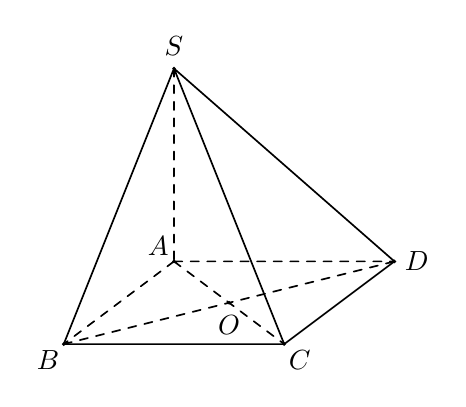
\begin{tikzpicture}[line join=round, line cap=round, line width=0.6pt, scale=0.7]
		\coordinate (A) at (0,0);
		\coordinate (D) at (4,0);
		\coordinate (B) at (-2,-1.5);
		\coordinate (C) at (2,-1.5);
		\coordinate (O) at (1,-0.75);
		\coordinate (S) at (0,3.5);
		\draw[dashed] (A)--(D) (A)--(B) (A)--(C) (B)--(D) (S)--(A) ;
		\draw (S)--(B)--(C)--(D)--cycle (S)--(C);
		\foreach \p/\pos in {S/90, A/135, B/-135, C/-45, D/0, O/-90}
		\fill (\p) circle (1pt) node[shift={(\pos:8pt)}] {$\p$};
	\end{tikzpicture}
	}
	
	\loigiai{
		\begin{itemize}
			\item Ta có $SA \perp (ABCD) \Rightarrow (SAC) \perp (ABCD)$. Do đó góc nhị diện $[S; AC; B] = 90^\circ$, mệnh đề A đúng.
			\item Vì đáy $ABCD$ là hình thoi nên $BD \perp AC$. Lại có $BD \perp SA$ nên $BD \perp (SAC) \Rightarrow (SBD) \perp (SAC)$, mệnh đề D đúng.
			\item Góc nhị diện $[S; BD; A]$ có cạnh nhị diện là $BD$. Vì $(SAC) \perp BD$ cắt $BD$ tại $O$, $OS \subset (SBD)$ và $OA \subset (ABCD)$ nên phẳng góc của nhị diện này là $\widehat{SOA}$. Mệnh đề B đúng.
			\item  Góc phẳng nhị diện $[S; BD; C]$ là $\widehat{SOC}$. Dễ thấy  $\widehat{SOC} \neq \widehat{SOA}$. Nên mệnh đề C sai.
		\end{itemize}
	}
\end{ex}

\begin{ex}%[2D4H2-2]
	Ta có  $\displaystyle\int\limits_{-1}^1 |e^x - 1| \mathrm{\,d}x = ae + b\mathrm{e}^{-1} + c$ với $a, b, c \in \mathbb{Z}$. Tính giá trị của biểu thức $a + b + c$.
	\choice
	{$3$}
	{$2$}
	{\True $0$}
	{$-2$}
	\loigiai{
		Ta có $e^x - 1 \ge 0 \Leftrightarrow x \ge 0$.\\
		Do đó
		{\allowdisplaybreaks
			\begin{eqnarray*}
				\displaystyle\int\limits_{-1}^1 |e^x - 1| \mathrm{\,d}x 
				&=& \displaystyle\int\limits_{-1}^0 (1 - e^x) \mathrm{\,d}x + \displaystyle\int\limits_0^1 (e^x - 1) \mathrm{\,d}x\\
				&=& (x - e^x) \Big|_{-1}^0 + (e^x - x) \Big|_0^1\\
				&=& e + \mathrm{e}^{-1} - 2.
		\end{eqnarray*}}
		Đồng nhất hệ số, ta được $a = 1, b = 1, c = -2$.\\
		Vậy $a + b + c = 1 + 1 - 2 = 0$.
	}
\end{ex}

\begin{ex}%[2H5H1-2]
	Trong không gian với hệ tọa độ $Oxyz$, mặt phẳng $(P)$ chứa trục $Ox$ và vuông góc với mặt phẳng $(\alpha)\colon 2x - 3y + 4z - 5 = 0$ có phương trình là
	\choice
	{\True $4y + 3z = 0$}
	{$4y - 3z = 0$}
	{$3x + 2y = 0$}
	{$3x + 4y - 1 = 0$}
	\loigiai{
		Mặt phẳng $(P)$ chứa trục $Ox$ nên nhận $\vec{i} = (1; 0; 0)$ làm một vectơ chỉ phương.\\
		Mặt phẳng $(P)$ vuông góc với $(\alpha)$ nên nhận vectơ pháp tuyến $\vec{n}_\alpha = (2; -3; 4)$ làm một vectơ chỉ phương.\\
		Một vectơ pháp tuyến của $(P)$ là $\vec{n}_P = \left[\vec{i}, \vec{n}_\alpha\right] = (0; -4; -3) = -1(0; 4; 3)$.\\
		Vì $(P)$ chứa $Ox$ nên $(P)$ đi qua gốc tọa độ $O(0;0;0)$.\\
		Phương trình mặt phẳng $(P)\colon 0(x - 0) + 4(y - 0) + 3(z - 0) = 0 \Leftrightarrow 4y + 3z = 0$.
	}
\end{ex}

\begin{ex}%[2H5H2-5]
	Trong không gian với hệ tọa độ $Oxyz$, cho mặt phẳng $(P)\colon 2x + y - z - 1 = 0$. Đường thẳng nào dưới đây song song với mặt phẳng $(P)$?
	\choice
	{$\dfrac{x - 1}{-1} = \dfrac{y + 3}{-3} = \dfrac{z + 1}{1}$}
	{$\dfrac{x + 1}{2} = \dfrac{y - 3}{1} = \dfrac{z - 1}{-1}$}
	{\True $\dfrac{x + 1}{-1} = \dfrac{y - 2}{3} = \dfrac{z}{1}$}
	{$\dfrac{x + 1}{-1} = \dfrac{y - 2}{2} = \dfrac{z}{1}$}
	\loigiai{
		Mặt phẳng $(P)$ có vectơ pháp tuyến $\vec{n}_P = (2; 1; -1)$.\\
		Xét đường thẳng ở phương án C:
		Đường thẳng này có vectơ chỉ phương $\vec{u} = (-1; 3; 1)$ và đi qua điểm $M(-1; 2; 0)$.\\
		Ta có $\vec{u} \cdot \vec{n}_P = -1 \cdot 2 + 3 \cdot 1 + 1 \cdot (-1) = 0 \Rightarrow \vec{u} \perp \vec{n}_P$.\\
		Thay tọa độ điểm $M(-1; 2; 0)$ vào phương trình $(P)$: $2(-1) + 2 - 0 - 1 = -1 \neq 0$, suy ra $M \notin (P)$.\\
		Vậy đường thẳng ở đáp án C song song với mặt phẳng $(P)$.
	}
\end{ex}

\begin{ex}%[1D2H2-4]
	Cho cấp số cộng $(u_n)$, biết $u_2 = 4; u_6 = 8$. Tìm số hạng thứ 100 của cấp số cộng đó.
	\choice
	{$106$}
	{\True $102$}
	{$100$}
	{$104$}
	\loigiai{
		Gọi $u_1$ là số hạng đầu và $d$ là công sai của cấp số cộng.\\
		Theo giả thiết ta có hệ phương trình
		$\heva{&u_2 = 4 \\ &u_6 = 8} \Leftrightarrow \heva{&u_1 + d = 4 \\ &u_1 + 5d = 8} \Leftrightarrow \heva{&u_1=3\\&d=1.}$\\
		Số hạng thứ 100 của cấp số cộng là $u_{100} = u_1 + 99d = 3 + 99 \cdot 1 = 102$.
	}
\end{ex}

\begin{ex}%[1D1N5-3]
	Tập nghiệm của phương trình $\cos x = -1$ là
	\choice
	{$S = \left\{\dfrac{-\pi}{3} + k2\pi, k \in \mathbb{Z}\right\}$}
	{\True $S = \{\pi + k2\pi, k \in \mathbb{Z}\}$}
	{$S = \left\{\dfrac{\pi}{2} + k2\pi, k \in \mathbb{Z}\right\}$}
	{$S = \left\{\dfrac{-\pi}{2} + k2\pi, k \in \mathbb{Z}\right\}$}
	\loigiai{
		Ta có $\cos x = -1 \Leftrightarrow x = \pi + k2\pi \quad (k \in \mathbb{Z})$.\\
		Vậy tập nghiệm của phương trình là $S = \{\pi + k2\pi, k \in \mathbb{Z}\}$.
	}
\end{ex}

\begin{ex}%[2D1N5-1]
	\immini[thm]{
	Đường cong trong hình bên là đồ thị của hàm số nào dưới đây?
	\choice
	{$y = -x^3 + 3x - 4$}
	{$y = -x^3 + 3x^2 + 4$}
	{\True $y = -x^3 + 3x^2 - 4$}
	{$y = x^3 + 3x^2 - 4$}
	}{
	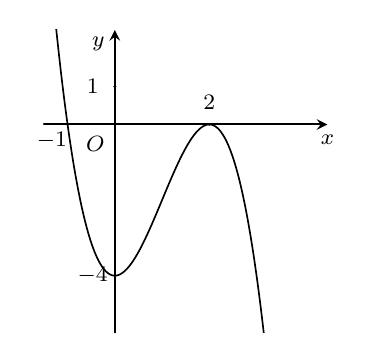
\begin{tikzpicture}[>=stealth, line join=round, line cap=round, every node/.style={font=\footnotesize}, declare function={f(\x)=-\x*\x*\x + 3*\x*\x - 4; xmin=-1.5; xmax=4.5; ymin=-5.5; ymax=2.5;},scale=0.6, yscale=0.8]
		
		\draw[-stealth, line width=0.7pt] (xmin, 0) -- (xmax, 0) node[below] {$x$};
		\draw[-stealth, line width=0.7pt] (0, ymin) -- (0, ymax) node[shift={(-6pt,-5pt)}] {$y$};
		
		\fill (0,0) circle (1pt) node[shift={(-135:10pt)}] {$O$};
		
		\begin{scope}
			\clip (xmin, ymin) rectangle (xmax, ymax);
			\draw[line width=0.6pt, smooth, samples=300, domain=xmin:xmax] plot (\x, {f(\x)});
		\end{scope}
		
		\foreach \x/\pos in {-1/-135,  2/90} {
			\fill (\x, 0) circle (1pt) node[shift={(\pos:8pt)}] {$\x$};
		}
		
		\foreach \y/\pos in {1/180, -4/-180} {
			\fill (0, \y) circle (1pt) node[shift={(\pos:8pt)}] {$\y$};
		}
		
	\end{tikzpicture}
	}
	
	\loigiai{
		Dựa vào đồ thị, ta thấy hệ số $a < 0$ nên loại phương án D.\\
		Đồ thị hàm số cắt trục tung tại điểm có tung độ bằng $-4$, do đó $y(0) = -4$ nên loại phương án B.\\
		Đồ thị hàm số đi qua điểm $(2; 0)$. Ta thay $x = 2$ vào các hàm số còn lại
		\begin{itemize}
			\item Với $y = -x^3 + 3x - 4$, ta có $y(2) = -2^3 + 3 \cdot 2 - 4 = -6 \neq 0$ (loại).
			\item Với $y = -x^3 + 3x^2 - 4$, ta có $y(2) = -2^3 + 3 \cdot 2^2 - 4 = -8 + 12 - 4 = 0$ (thỏa mãn).
		\end{itemize}
		Vậy hàm số cần tìm là $y = -x^3 + 3x^2 - 4$.
	}
\end{ex}

\begin{ex}%[1D6N4-3]
	Tập nghiệm của bất phương trình $\log_{\frac{1}{2}}(x-2) > -5$ là
	\choice
	{\True $(2; 34)$}
	{$(-\infty; 34)$}
	{$(2; +\infty)$}
	{$(34; +\infty)$}
	\loigiai{
		Điều kiện: $x - 2 > 0 \Leftrightarrow x > 2$.\\
		Bất phương trình đã cho tương đương với
		{\allowdisplaybreaks
			\begin{eqnarray*}
			&&x - 2 < \left(\dfrac{1}{2}\right)^{-5}\\
			&\Leftrightarrow& x - 2 < 32\\
			&\Leftrightarrow& x < 34.
		\end{eqnarray*}}
		Kết hợp với điều kiện, ta được tập nghiệm của bất phương trình là $(2; 34)$.
	}
\end{ex}

\cauds

\begin{ex}%[2H5V3-4]
	Trong không gian với hệ tọa độ $Oxyz$, cho hai mặt cầu $(S_1)$ và $(S_2)$ có tâm lần lượt là $I(-4;-5;0)$ và $J(6;8;3)$.
	Mặt cầu $(S_2)$ cắt mặt phẳng $(Oxy)$ theo thiết diện là một đường tròn có bán kính $r_2 = 4$.
	Mặt cầu $(S_1)$ có bán kính $R_1 = 4$.
	Một điểm $M$ có tọa độ cố định $M(1;0;10)$.
	Một điểm $C$ di chuyển từ $M$ đến một điểm bất kỳ thuộc mặt cầu $(S_1)$ hoặc $(S_2)$.
	Năng lượng tiêu hao khi di chuyển của điểm $C$ được xác định bởi hàm số $E(s) = \dfrac{1}{12} \cdot s^2$ (đơn vị năng lượng), trong đó $s$ là độ dài quãng đường di chuyển.
	Xét tính đúng sai của các mệnh đề sau.
	\choiceTF
	{\True Bán kính của mặt cầu $(S_2)$ bằng $5$}
	{Năng lượng tối thiểu để điểm $C$ di chuyển từ $M$ đến bề mặt khối cầu tâm $I$ là $\dfrac{175 - 50\sqrt{6}}{12}$ (đơn vị năng lượng)}
	{\True Gọi $A$ và $B$ lần lượt là hai điểm bất kỳ thuộc mặt cầu $(S_1)$ và $(S_2)$. Độ dài lớn nhất của đoạn $AB$ có giá trị lớn hơn $25$}
	{\True Năng lượng tối thiểu để điểm $C$ di chuyển vào bên trong khối cầu $(S_2)$ nhỏ hơn năng lượng tối thiểu để điểm $C$ di chuyển vào bên trong khối cầu $(S_1)$}
	\loigiai{
		Ta có $I(-4;-5;0)$, $J(6;8;3)$, $M(1;0;10)$, $R_1 = 4$.
		\begin{center}
			\begin{tikzpicture}[,scale=0.8,
				>=stealth, 
				line join=round, 
				line cap=round, 
				every node/.style={font=\normalsize},
				declare function={
					R1=1.5; 
					R2=1.5; 
					xI=-2; yI=1.5; 
					xJ=2.5; yJ=1.7; 
					xM=0.5; yM=5; 
					xH=2.5; yH=-0.5; 
					aElip=1.2; bElip=0.25;
				}
				]
				
				\path
				(xI, yI) coordinate (I)
				(xJ, yJ) coordinate (J)
				(xM, yM) coordinate (M)
				(xH, yH) coordinate (H)
				(xH+aElip, yH) coordinate (E)
				;
				
				\draw[dash pattern=on 2.5pt off 1.5pt, line width=0.6pt] (I) + (R1,0) arc (0:180:R1 and 0.3);
				\draw[line width=0.6pt] (I) + (-R1,0) arc (180:360:R1 and 0.3);
				\draw[line width=0.6pt] (I) circle (R1);
				\node at (-3.3, 3) {$(S_1)$};
				
				\draw[dash pattern=on 2.5pt off 1.5pt, line width=0.6pt] (J) + (R2,0) arc (0:180:R2 and 0.3);
				\draw[line width=0.6pt] (J) + (-R2,0) arc (180:360:R2 and 0.3);
				\draw[line width=0.6pt] (J) circle (R2);
				\node at (4.3, 3.2) {$(S_2)$};
				
				\draw[line width=0.6pt] (-0.5, -1.2) -- (5, -1.2) -- (7.5, 0.5) -- (2, 0.5) -- cycle;
				\node at (7.8, -0.6) {$(Oxy)$};
				
				\draw[dashed, line width=0.6pt] (H) ellipse (aElip and bElip);
				
				\draw[dashed, line width=0.6pt] (I) -- (M);
				\draw[dashed, line width=0.6pt] (J) -- (M);
				\draw[dashed, line width=0.6pt] (J) -- (H);
				\draw[dashed, line width=0.6pt] (H) -- (E) node[right, font=\normalsize] {$r_2 = 4$};
				
				\path pic[draw, line width=0.6pt, angle radius=5pt]{right angle=J--H--E};
				
				\fill (I) circle (1pt) node[below=2pt] {$I$};
				\fill (J) circle (1pt) node[right=2pt] {$J$};
				\fill (M) circle (1pt) node[right=2pt] {$M(1; 0; 10)$};
				\fill (H) circle (1pt);
				
			\end{tikzpicture}
		\end{center}
		\begin{itemchoice}
			\itemch $\mathrm{d}(J, (Oxy)) = |3| = 3$.\\
			$R_2^2 = r_2^2 + d^2 = 4^2 + 3^2 = 25$.\\
			Suy ra $R_2 = 5$.
			\itemch $MI = \sqrt{(1+4)^2 + (0+5)^2 + (10-0)^2} = \sqrt{150} = 5\sqrt{6}$.\\
			$S_{\min} = MI - R_1 = 5\sqrt{6} - 4$.\\
			$E_{\min} = \dfrac{1}{12} \cdot (5\sqrt{6} - 4)^2 = \dfrac{166 - 40\sqrt{6}}{12}$.
			\itemch $IJ = \sqrt{(6+4)^2 + (8+5)^2 + (3-0)^2} = \sqrt{278}$.\\	
			$AB_{\max} = IJ + R_1 + R_2 = \sqrt{278} + 9 \approx 25{,}67 > 25$.
			\itemch $S_1 = 5\sqrt{6} - 4 \approx 8{,}25$.\\
			$MJ = \sqrt{(1-6)^2 + (0-8)^2 + (10-3)^2} = \sqrt{138}$.\\
			$S_2 = \sqrt{138} - 5 \approx 6{,}75$.\\
			Vì $S_2 < S_1$ và $E(s) = \dfrac{1}{12} \cdot s^2$ tăng với $s > 0$ nên $E_2 < E_1$.
		\end{itemchoice}
	}
\end{ex}

\begin{ex}%[2D5V2-4]
	Trong một nghiên cứu về hai loại thuốc A và B, xác suất thuốc A gây tác dụng phụ là $20\%$; xác suất thuốc B gây tác dụng phụ là $10\%$.
	Một bệnh nhân được chọn ngẫu nhiên để dùng một trong hai loại thuốc (xác suất chọn mỗi loại thuốc là $50\%$).
	\choiceTF
	{\True Xác suất để bệnh nhân bị tác dụng phụ khi dùng thuốc A là $20\%$}
	{\True Xác suất để bệnh nhân bị tác dụng phụ khi được chọn ngẫu nhiên dùng một trong hai loại thuốc là $0{,}15$}
	{ Nếu biết bệnh nhân không bị tác dụng phụ, xác suất để bệnh nhân đó dùng thuốc B là $\dfrac{7}{17}$}
	{Xác suất để bệnh nhân dùng thuốc A và không bị tác dụng phụ là $0{,}425$}
	\loigiai{
		Gọi $T$ là biến cố bệnh nhân bị tác dụng phụ.\\
		Ta có $\mathrm{P}(A) = \mathrm{P}(B) = 0{,}5$; $\mathrm{P}(T|A) = 0{,}2$; $\mathrm{P}(T|B) = 0{,}1$.
		\begin{center}
			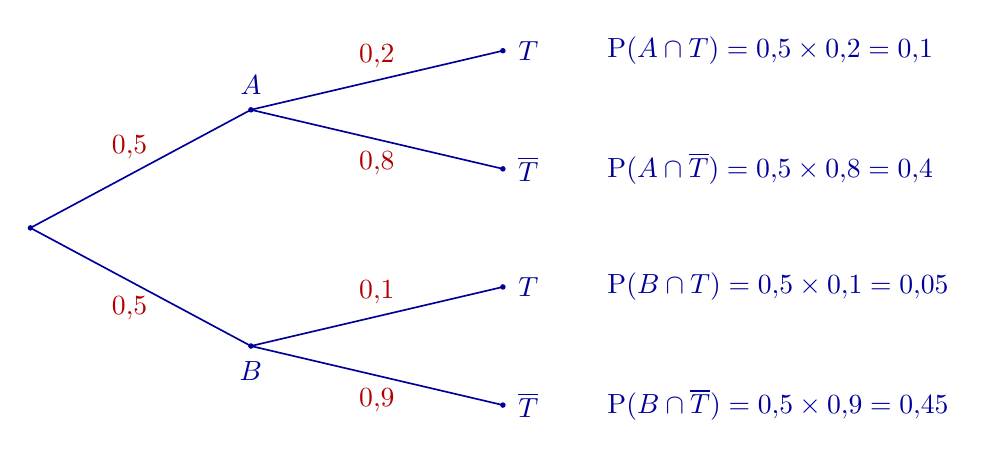
\begin{tikzpicture}[
				declare function={
					dx=2.8; 
					dy=1.5; 
					dx2=3.2; 
					dy2=0.75; 
					dx3=1.2;
				},
				>=stealth,
				line width=0.6pt,
				every node/.style={font=\normalsize, text=blue!60!black}
				]
				
				\path 
				(0,0) coordinate (O)
				(dx, dy) coordinate (A)
				(dx, -dy) coordinate (B)
				({dx+dx2}, {dy+dy2}) coordinate (TA)
				({dx+dx2}, {dy-dy2}) coordinate (TbA)
				({dx+dx2}, {-dy+dy2}) coordinate (TB)
				({dx+dx2}, {-dy-dy2}) coordinate (TbB)
				;
				
				\draw[blue!60!black] (O) -- (A) node[pos=0.45, above=2pt, text=red!70!black] {$0{,}5$};
				\draw[blue!60!black] (O) -- (B) node[pos=0.45, below=2pt, text=red!70!black] {$0{,}5$};
				
				\draw[blue!60!black] (A) -- (TA) node[pos=0.5, above=1pt, text=red!70!black] {$0{,}2$};
				\draw[blue!60!black] (A) -- (TbA) node[pos=0.5, below=1pt, text=red!70!black] {$0{,}8$};
				
				\draw[blue!60!black] (B) -- (TB) node[pos=0.5, above=1pt, text=red!70!black] {$0{,}1$};
				\draw[blue!60!black] (B) -- (TbB) node[pos=0.5, below=1pt, text=red!70!black] {$0{,}9$};
				
				\foreach \p in {O, A, B, TA, TbA, TB, TbB} {
					\fill[blue!60!black] (\p) circle (1pt);
				}
				
				\node[above=2pt] at (A) {$A$};
				\node[below=2pt] at (B) {$B$};
				\node[right=2pt] at (TA) {$T$};
				\node[right=2pt] at (TbA) {$\overline{T}$};
				\node[right=2pt] at (TB) {$T$};
				\node[right=2pt] at (TbB) {$\overline{T}$};
				
				\node[right] at ({dx+dx2+dx3}, {dy+dy2}) {$\mathrm{P}(A \cap T) = 0{,}5 \times 0{,}2 = 0{,}1$};
				\node[right] at ({dx+dx2+dx3}, {dy-dy2}) {$\mathrm{P}(A \cap \overline{T}) = 0{,}5 \times 0{,}8 = 0{,}4$};
				\node[right] at ({dx+dx2+dx3}, {-dy+dy2}) {$\mathrm{P}(B \cap T) = 0{,}5 \times 0{,}1 = 0{,}05$};
				\node[right] at ({dx+dx2+dx3}, {-dy-dy2}) {$\mathrm{P}(B \cap \overline{T}) = 0{,}5 \times 0{,}9 = 0{,}45$};
				
			\end{tikzpicture}
		\end{center}
		\begin{itemchoice}
			\itemch $\mathrm{P}(T|A) = 0{,}2 = 20\%$.
			\itemch $\mathrm{P}(T) = 0{,}1 + 0{,}05 = 0{,}15$.
			\itemch $\mathrm{P}(B|\overline{T}) = \dfrac{\mathrm{P}(B \cap \overline{T})}{\mathrm{P}(\overline{T})} = \dfrac{0{,}45}{0{,}4 + 0{,}45} = \dfrac{0{,}45}{0{,}85} = \dfrac{9}{17} \neq \dfrac{7}{17}$.
			\itemch$\mathrm{P}(A \cap \overline{T}) = 0{,}4 \neq 0{,}425$.
			
		\end{itemchoice}
		
	}
\end{ex}

\begin{ex}%[2D1V3-6]
	Một hạt chuyển động dọc theo trục $Ox$. Vị trí của hạt (đơn vị: mét) tại thời điểm $t$ (giây) được xác định bởi hàm số $x(t) = 20t^2\mathrm{e}^{-0{,}5t}$ (m), (với $t \ge 0$). Xét tính đúng sai của các mệnh đề sau:
	\choiceTF
	{Vận tốc xuất phát của hạt tại thời điểm $t = 0$ là $20\text{m/s}$}
	{\True Trong suốt quá trình chuyển động, hạt chỉ đổi chiều chuyển động đúng một lần duy nhất}
	{\True Khoảng cách xa nhất mà hạt đạt được so với gốc tọa độ $O$ là $320\mathrm{e}^{-2}$ (m)}
	{Tổng quãng đường hạt đi được không quá $320\mathrm{e}^{-2}$ (m)}
	\loigiai{
		Ta có $x(t) = 20t^2\mathrm{e}^{-0{,}5t}$, $t \ge 0$.\\
		Vận tốc của hạt $v(t) = x'(t)$.
		{\allowdisplaybreaks
			\begin{eqnarray*}
				v(t) &=& \left( 20t^2\mathrm{e}^{-0{,}5t} \right)' = 20 \left( t^2\mathrm{e}^{-0{,}5t} \right)' \\
				&=& 20 \left( 2t \mathrm{e}^{-0{,}5t} + t^2 \cdot (-0{,}5) \mathrm{e}^{-0{,}5t} \right) \\
				&=& 20 \mathrm{e}^{-0{,}5t} \left( 2t - \dfrac{1}{2}t^2 \right) = 10t\mathrm{e}^{-0{,}5t}(4 - t).
		\end{eqnarray*}}
		
		\begin{itemchoice}
			\itemch $v(0) = 10 \cdot 0 \cdot e^0 \cdot (4 - 0) = 0$ (m/s).
			Vận tốc xuất phát bằng $0\text{ m/s}$.
			\itemch $v(t) = 0 \Leftrightarrow 10t\mathrm{e}^{-0{,}5t}(4 - t) = 0 \Leftrightarrow \hoac{&t = 0 \\ &t = 4.}$\\
			Với $0 < t < 4$ thì $v(t) > 0$ (hạt chuyển động theo chiều dương).\\
			Với $t > 4$ thì $v(t) < 0$ (hạt chuyển động theo chiều âm).
			Vậy hạt đổi chiều đúng một lần tại $t = 4$.
			\itemch Vì $x(t) \ge 0$ với $t \ge 0$ nên khoảng cách từ hạt đến gốc tọa độ $O$ là $|x(t)| = x(t)$.\\
			Từ câu b) hàm $x(t)$ tăng trên $(0; 4)$ và giảm trên $(4; +\infty)$.\\
			Do đó $x(t)$ đạt giá trị lớn nhất tại $t = 4$.\\
			Khi đó $x(4) = 20 \cdot 4^2 \cdot \mathrm{e}^{-0{,}5 \cdot 4} = 20 \cdot 16 \cdot \mathrm{e}^{-2} = 320\mathrm{e}^{-2}$ (m).\\
			Vậy khoảng cách xa nhất so với $O$ là $320\mathrm{e}^{-2}$ (m).
			\itemch Ta có $x(0) = 0, x(4) = 320\mathrm{e}^{-2}, \lim\limits_{t \to +\infty} x(t) = \lim\limits_{t \to +\infty} 20t^2\mathrm{e}^{-0{,}5t} = 0$.\\
			Từ $t = 0$ đến $t = 4$, hạt đi từ $0$ đến $320\mathrm{e}^{-2}$ nên quãng đường $S_1 = 320\mathrm{e}^{-2}$.\\
			Từ $t = 4$ đến $t \to +\infty$, hạt đi từ $320\mathrm{e}^{-2}$ về gần $0$ nên quãng đường $S_2 = 320\mathrm{e}^{-2}$.\\
			Vậy tổng quãng đường $S = S_1 + S_2 = 320\mathrm{e}^{-2} + 320\mathrm{e}^{-2} = 640\mathrm{e}^{-2}$.\\
			Do đó $S = 640\mathrm{e}^{-2} > 320\mathrm{e}^{-2}$ nên mệnh đề d) sai.
		\end{itemchoice}
	}
\end{ex}

\begin{ex}%[2D1V5-1]
	Cho hàm số $y = \dfrac{x^2+x-6}{x+1}$ có đồ thị là đường cong $(C)$. Giả sử $A, B$ là $2$ điểm thuộc $2$ nhánh của đồ thị $(C)$ sao cho $AB$ song song với trục hoành. Xét tính đúng sai của các mệnh đề sau.
	\choiceTF
	{\True Đồ thị $(C)$ có tâm đối xứng là điểm $I(-1;-1)$}
	{Có $2$ tiếp tuyến của đồ thị $(C)$ song song với đường thẳng $d\colon y=7x+18$}
	{Giá trị nhỏ nhất của đoạn thẳng $AB$ bằng $2\sqrt{5}$}
	{\True Gọi $(K)$ là hình phẳng giới hạn bởi đồ thị hàm số $y=\dfrac{x^2+x-6}{x+1}-x$, trục hoành, trục tung và đường thẳng $x=m,m>0$. Gọi $V$ là thể tích khối tròn xoay tạo thành khi quay $(K)$ quanh trục hoành. Khi đó $\lim\limits_{m \to +\infty} V = 36\pi$}
	\loigiai{
		Tập xác định $\mathscr{D} = \mathbb{R} \setminus \{-1\}$.\\
		Ta có $y = \dfrac{x^2+x-6}{x+1} = \dfrac{x(x+1) - 6}{x+1} = x - \dfrac{6}{x+1}$.\\
		Đạo hàm $y' = 1 + \dfrac{6}{(x+1)^2}$.
		\begin{itemchoice}
			\itemch Đồ thị $(C)$ có tiệm cận đứng là $x = -1$ và tiệm cận xiên là $y = x$.\\
			Giao điểm của hai đường tiệm cận là nghiệm của hệ $\heva{&x = -1 \\ &y = x} \Leftrightarrow \heva{&x = -1 \\ &y = -1.}$\\
			Vậy tâm đối xứng của đồ thị $(C)$ là $I(-1; -1)$.
			\itemch Tiếp tuyến song song với đường thẳng $d\colon y = 7x+18$ nên có hệ số góc $k = 7$.\\
			Ta có phương trình
			{\allowdisplaybreaks
				\begin{eqnarray*}
				y' = 7 &\Leftrightarrow& 1 + \dfrac{6}{(x+1)^2} = 7\\ &\Leftrightarrow& \dfrac{6}{(x+1)^2} = 6\\
				&\Leftrightarrow& (x+1)^2 = 1 \\
				&\Leftrightarrow& \hoac{&x = 0 \\ &x = -2.}
			\end{eqnarray*}}
			Với $x=0$, tiếp điểm có tọa độ $(0; -6)$.
			Phương trình tiếp tuyến là $y = 7x - 6$ (nhận).\\
			Với $x=-2$, tiếp điểm có tọa độ $(-2; 4)$. Phương trình tiếp tuyến là $y = 7(x+2) + 4 = 7x + 18$ (loại).\\
			Vậy chỉ có đúng $1$ tiếp tuyến thỏa mãn.
			\itemch Do $AB$ song song với trục hoành nên $A, B$ có cùng tung độ $m$.\\
			Hoành độ $x_A, x_B$ là $2$ nghiệm phân biệt của phương trình 
			{\allowdisplaybreaks
				\begin{eqnarray*}
				&&\dfrac{x^2+x-6}{x+1} = m\\
				&\Leftrightarrow& x^2 + x - 6 = m(x+1)\\ 
				&\Leftrightarrow& x^2 + (1-m)x - m - 6 = 0\ (\text{với } x \neq -1).
			\end{eqnarray*}}
			Để có $2$ điểm nằm trên $2$ nhánh của đồ thị thì phương trình trên phải có hai nghiệm $x_A, x_B$ thỏa mãn $x_A < -1 < x_B$.\\
			Nghĩa là $(x_A + 1)(x_B + 1) < 0 \Leftrightarrow x_A x_B + (x_A + x_B) + 1 < 0$.\\
			Áp dụng định lý Viète: $-(m+6) - (1-m) + 1 < 0 \Leftrightarrow -6 < 0$ (luôn đúng).\\
			Khi đó, độ dài $AB$ là $AB = |x_A - x_B| = \sqrt{(x_A+x_B)^2 - 4x_Ax_B}$.
			{\allowdisplaybreaks
				\begin{eqnarray*} 
					AB &=& \sqrt{(m-1)^2 - 4(-m-6)} \\
					&=& \sqrt{m^2 - 2m + 1 + 4m + 24} \\
					&=& \sqrt{m^2 + 2m + 25} \\
					&=& \sqrt{(m+1)^2 + 24} \ge \sqrt{24} = 2\sqrt{6}.
			\end{eqnarray*}}
			Giá trị nhỏ nhất của $AB$ là $2\sqrt{6}$.
			\itemch Hàm số $f(x) = \dfrac{x^2+x-6}{x+1} - x = \dfrac{-6}{x+1}$.\\
			Thể tích khối tròn xoay là $V = \pi \displaystyle\int\limits_{0}^{m} \left( \dfrac{-6}{x+1} \right)^2 \mathrm{d}x = 36\pi \displaystyle\int\limits_{0}^{m} \dfrac{1}{(x+1)^2} \mathrm{d}x$.\\
			$V = 36\pi \left( \dfrac{-1}{x+1} \right) \bigg|_0^m = 36\pi \left( 1 - \dfrac{1}{m+1} \right)$.\\
			Ta có $\lim\limits_{m \to +\infty} V = \lim\limits_{m \to +\infty} 36\pi \left( 1 - \dfrac{1}{m+1} \right) = 36\pi$.
		\end{itemchoice}
	}
\end{ex}

\caukq
\newpage
\begin{ex}%[2D4C3-5]
	\immini[thm]{
	Bác Tuấn trang trí bức tường hình vuông $ABCD$ có $AB=4m$ như hình vẽ bằng cách sơn màu. Trong đó, bốn đường cong $AQB, APD, BEC, CFD$ đều là đường parabol có các đỉnh lần lượt là $Q, P, E, F$. Biết rằng trục đối xứng của mỗi Parabol trùng với một trục đối xứng của hình vuông $ABCD$. Cho biết $OE = OF = OP = OQ = 1m$. Phần diện tích giới hạn bởi bốn đường Parabol nêu trên (phần gạch chéo) được sơn màu đỏ với chi phí $500$ nghìn đồng cho mỗi mét vuông. Phần diện tích còn lại của bức tường được sơn màu trắng với chi phí $300$ nghìn đồng cho mỗi mét vuông. Tính tổng số tiền (đơn vị: nghìn đồng) bác Tuấn cần để hoàn thành việc sơn bức tường đó. (Kết quả làm tròn đến hàng đơn vị).
	}{
	\begin{tikzpicture}[
		>=stealth, line join=round, line cap=round, scale=1,
		every node/.style={font=\footnotesize}
		]
		% ==========================================
		% 1. BẢNG ĐIỀU KHIỂN THAM SỐ (TỰ ĐỘNG HÓA 100%)
		% ==========================================
		\def\s{3} % <s> = Nửa cạnh hình vuông
		\def\v{1} % <v> = Khoảng cách từ tâm O đến đỉnh Parabol (Điều kiện: v < s)
		
		% ==========================================
		% 2. TÍNH TOÁN CÁC MỐC GIẢI TÍCH
		% ==========================================
		\pgfmathsetmacro{\k}{(\s+\v)/(\s*\s)}       % Hệ số mở k
		\pgfmathsetmacro{\d}{-(\s*\v)/(\s+\v)}      % Hoành độ giao điểm trên đường chéo (mang dấu âm)
		\pgfmathsetmacro{\c}{\s*sqrt(\v/(\s+\v))}   % Hoành độ giao điểm trên trục tọa độ
		
		% KHAI BÁO DUY NHẤT 1 HÀM SỐ LÕI
		\tikzset{
			declare function={
				f(\x) = \k*\x*\x - \v; % Hàm lõi: Parabol mở lên trên
			}
		}
		
		% ==========================================
		% 3. XUẤT ĐỒ THỊ BẰNG 1 HÀM SỐ
		% ==========================================
		% Vẽ khung hình vuông
		\draw[line width=0.6pt] (-\s,-\s) rectangle (\s,\s);
		
		% Vòng lặp xoay 4 hướng
		\foreach \i in {0, 90, 180, 270} {
			\begin{scope}[rotate=\i]
				% TÔ MÀU 1 CÁNH HOA: Nối 4 cung bằng cách gọi lại hàm f(x)
				\fill[pattern={Lines[angle=45, distance=3pt, line width=0.3pt]}]
				(-\s,\s) 
				% Biên 1 & 2: Dùng f(x) để vẽ Parabol ngang (Đảo vị trí hoành - tung)
				-- plot[domain=\s:\c, smooth, samples=30] ({-f(\x)}, \x)
				-- plot[domain=\c:-\d, smooth, samples=30] ({f(\x)}, \x)
				% Biên 3 & 4: Dùng f(x) để vẽ Parabol dọc như bình thường
				-- plot[domain=\d:-\c, smooth, samples=30] (\x, {-f(\x)}) 
				-- plot[domain=-\c:-\s, smooth, samples=30] (\x, {f(\x)})
				-- cycle;
				
				% VẼ ĐƯỜNG BIÊN PARABOL CHUẨN
				\draw[line width=0.6pt, smooth, samples=80, domain=-\s:\s] plot (\x, {f(\x)});
			\end{scope}
		}
		
		% ==========================================
		% 4. GẮN NHÃN TỰ ĐỘNG
		% ==========================================
		\foreach \x/\y/\vt/\ten in {
			-\s/\s/above left/A, 
			-\s/-\s/below left/B, 
			\s/-\s/below right/C, 
			\s/\s/above right/D%
		} \node[\vt=1pt] at (\x,\y) {${\ten}$};
		
		\foreach \x/\y/\vt/\ten in {
			0/0/below/O, 
			0/\v/below/E, 
			0/-\v/above/P, 
			-\v/0/right/F, 
			\v/0/left/Q%
		} \fill (\x,\y) circle (0.7pt) node[\vt=1pt] {${\ten}$};		\end{tikzpicture}
	}
	\shortans[oly]{$6129$}
	\loigiai{
		\begin{center}
			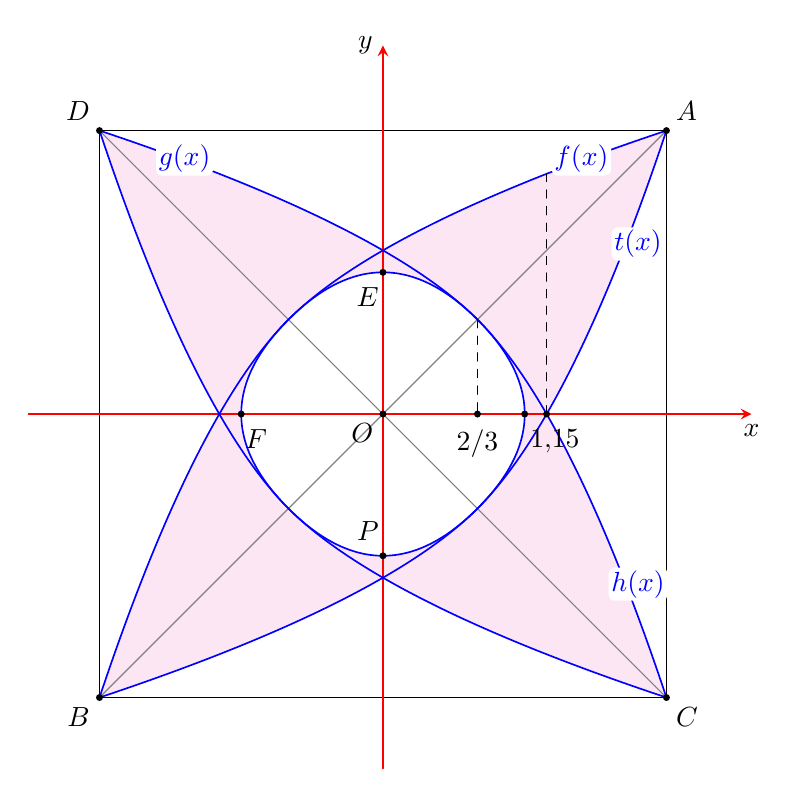
\begin{tikzpicture}[
				>=stealth, line join=round, line cap=round, scale=1.8,
				every node/.style={font=\normalsize},
				declare function={
					t(\x) = 0.75*\x*\x - 1;
					h(\x) = -0.75*\x*\x + 1;
					f(\x) = sqrt(4/3*(\x+1));
				}
				]
				\pgfmathsetmacro{\a}{2}
				\pgfmathsetmacro{\d}{2/3}
				\pgfmathsetmacro{\r}{2/sqrt(3)}
				
				% 1. TÔ MÀU VÙNG CÁNH HOA (MAGENTA) VÀ LÕI (TRẮNG)
				% Cánh hoa góc phần tư I (Petal A)
				\fill[magenta!10] plot[domain=-\d:\a, smooth, samples=100] (\x, {t(\x)}) -- plot[domain=\a:-\d, smooth, samples=100] ({t(\x)}, \x) -- cycle;
				% Cánh hoa góc phần tư II (Petal B)
				\fill[magenta!10] plot[domain=\d:-\a, smooth, samples=100] (\x, {t(\x)}) -- plot[domain=\a:-\d, smooth, samples=100] ({h(\x)}, \x) -- cycle;
				% Cánh hoa góc phần tư III (Petal C)
				\fill[magenta!10] plot[domain=\d:-\a, smooth, samples=100] (\x, {h(\x)}) -- plot[domain=-\a:\d, smooth, samples=100] ({h(\x)}, \x) -- cycle;
				% Cánh hoa góc phần tư IV (Petal D)
				\fill[magenta!10] plot[domain=-\d:\a, smooth, samples=100] (\x, {h(\x)}) -- plot[domain=-\a:\d, smooth, samples=100] ({t(\x)}, \x) -- cycle;
				
				% Lõi giữa màu trắng
				\fill[white] plot[domain=\d:-\d, smooth, samples=50] (\x, {h(\x)}) 
				-- plot[domain=\d:-\d, smooth, samples=50] ({t(\x)}, \x) 
				-- plot[domain=-\d:\d, smooth, samples=50] (\x, {t(\x)}) 
				-- plot[domain=-\d:\d, smooth, samples=50] ({h(\x)}, \x) 
				-- cycle;
				
				% 2. HÌNH VUÔNG VÀ ĐƯỜNG CHÉO
				\draw[line width=0.6pt] (-\a,-\a) rectangle (\a,\a);
				\draw[line width=0.4pt, gray] (-\a,-\a) -- (\a,\a);
				\draw[line width=0.4pt, gray] (-\a,\a) -- (\a,-\a);
				
				% 3. HỆ TRỤC TỌA ĐỘ
				\draw[-stealth, line width=0.7pt, red] (-2.5, 0) -- (2.6, 0) node[below, black] {$x$};
				\draw[-stealth, line width=0.7pt, red] (0, -2.5) -- (0, 2.6) node[left, black] {$y$};
				
				% 4. CÁC ĐƯỜNG PARABOL
				\draw[blue, line width=0.6pt, smooth, samples=150, domain=-\a:\a] plot (\x, {t(\x)});
				\draw[blue, line width=0.6pt, smooth, samples=150, domain=-\a:\a] plot (\x, {h(\x)});
				\draw[blue, line width=0.6pt, smooth, samples=150, domain=-\a:\a] plot ({t(\x)}, \x);
				\draw[blue, line width=0.6pt, smooth, samples=150, domain=-\a:\a] plot ({h(\x)}, \x);
				
				% 5. ĐƯỜNG GIÓNG VÀ ĐIỂM ĐÁNH DẤU
				\draw[dashed, line width=0.4pt] (\d, \d) -- (\d, 0);
				\node[below, shift={(0,-2pt)}] at (\d, 0) {$2/3$};
				
				\draw[dashed, line width=0.4pt] (\r, 0) -- (\r, {f(\r)});
				\node[below, shift={(3pt,-2pt)}] at (\r, 0) {$1{,}15$};
				
				\fill (0,1) circle (0.7pt);
				\fill (-1,0) circle (0.7pt);
				\fill (0,-1) circle (0.7pt);
				\fill (1,0) circle (0.7pt);
				\fill (\a,\a) circle (0.7pt);
				\fill (-\a,-\a) circle (0.7pt);
				\fill (\a,-\a) circle (0.7pt);
				\fill (-\a,\a) circle (0.7pt);
				\fill (0,0) circle (0.7pt);
				\fill (\d, 0) circle (0.7pt);
				\fill (\r, 0) circle (0.7pt);
				
				% 6. NHÃN ĐIỂM VÀ ĐỒ THỊ
				\node[above right] at (\a,\a) {$A$};
				\node[below left] at (-\a,-\a) {$B$};
				\node[below right] at (\a,-\a) {$C$};
				\node[above left] at (-\a,\a) {$D$};
				
				\node[below left, shift={(2pt,-2pt)}] at (0,1) {$E$};
				\node[below right, shift={(-2pt,-2pt)}] at (-1,0) {$F$};
				\node[above left, shift={(2pt,2pt)}] at (0,-1) {$P$};

				\node[below left] at (0,0) {$O$};
				
				\node[blue, fill=white, inner sep=1pt, rounded corners=2pt] at (1.4, 1.8) {$f(x)$};
				\node[blue, fill=white, inner sep=1pt, rounded corners=2pt] at (1.8, 1.2) {$t(x)$};
				\node[blue, fill=white, inner sep=1pt, rounded corners=2pt] at (1.8, -1.2) {$h(x)$};
				\node[blue, fill=white, inner sep=1pt, rounded corners=2pt] at (-1.4, 1.8) {$g(x)$};
				
			\end{tikzpicture}
		\end{center}
		Chọn hệ trục tọa độ $Oxy$ với gốc tọa độ $O$ trùng với tâm hình vuông $ABCD$ như hình vẽ.\\
		Khi đó, các đỉnh của hình vuông có tọa độ là $A(-2; 2)$, $B(-2; -2)$, $C(2; -2)$, $D(2; 2)$.\\
		Xét trên góc phần tư thứ I ($x \ge 0; y \ge 0$):
		\begin{itemize}
			\item Đồ thị hàm số $h(x)$ tương ứng với cung parabol $(BEC)$ có đỉnh $E(0; 1)$ và đi qua điểm $C(2; -2)$. Phương trình của $h(x)$ là $y = -\dfrac{3}{4}x^2 + 1$.
			\item Đồ thị hàm số $t(x)$ đối xứng với $h(x)$ qua $Ox$ nên phương trình của $t(x)$ là $y = \dfrac{3}{4}x^2 - 1$.
			\item Đồ thị hàm số $g(x)$ tương ứng với nhánh trên của parabol $(AQB)$. Vì $(AQB)$ và $(BEC)$ đối xứng nhau qua đường phân giác $y = x$, ta có
			$$x = -\dfrac{3}{4}g^2(x) + 1 \Rightarrow g(x) = \sqrt{-\dfrac{4}{3}(x-1)}.$$
		\end{itemize}
		Tìm các hoành độ giao điểm.
		\begin{itemize}
		\item Đồ thị $f(x)$ và $g(x)$ cắt nhau tại $x = 0$.	
		\item Đồ thị $g(x)$ và $h(x)$ cắt nhau tại $x = \dfrac{2}{3}$.
		\item Đồ thị $h(x)$ và $t(x)$ cắt nhau tại $x = \dfrac{2}{\sqrt{3}} \approx 1{,}15$.
		\end{itemize}
		Gọi $S_{\text{hoa}}$ là diện tích phần gạch chéo (gồm 4 cánh hoa bằng nhau). \\
		Ta có
		$$S_{\text{hoa}} = 4 \left[ \displaystyle\int\limits_{0}^{2/3} [f(x) - g(x)]\mathrm{d}x + \displaystyle\int\limits_{2/3}^{2/\sqrt{3}} [f(x) - h(x)]\mathrm{d}x + \displaystyle\int\limits_{2/\sqrt{3}}^{2} [f(x) - t(x)]\mathrm{d}x \right].$$
		Ta được $S_{\text{hoa}} \approx 6{,}646$ (m$^2$).\\
		Diện tích bức tường hình vuông là $S_{ABCD} = 4^2 = 16$ (m$^2$).\\
		Tổng số tiền bác Tuấn cần để hoàn thành việc sơn là
		$$\text{Tiền} = S_{\text{hoa}} \cdot 500 + (16 - S_{\text{hoa}}) \cdot 300 \approx 6129\text{ (nghìn đồng).}$$
	}
\end{ex}

\begin{ex}%[0D8C2-6]
	\immini[thm]{
	Bác Huy định tô màu hình vẽ là hình tròn được chia thành 5 phần $O, A, B, C, D$ bằng 6 màu khác nhau (mỗi phần tô một màu) sao cho hai phần hình cạnh nhau thì không được tô cùng màu (2 phần có chung biên được gọi là cạnh nhau: $C$ và $D$ được gọi là cạnh nhau; $C$ và $A$ gọi là không cạnh nhau...). Bác Huy có bao nhiêu cách tô màu thoả mãn yêu cầu trên?
	}{
	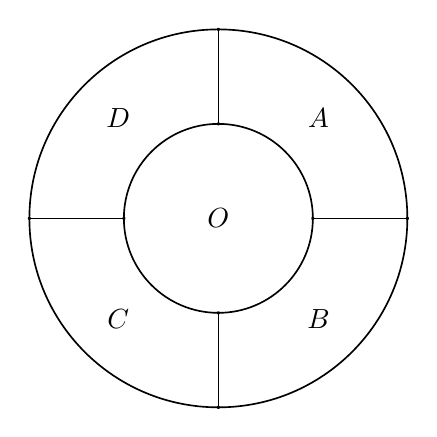
\begin{tikzpicture}[>=stealth, line join=round, line cap=round, every node/.style={font=\normalsize}, declare function={R=3; r=1.5; mid=(R+r)/2;},scale=0.8]
		
		\draw[line width=0.6pt] (0,0) circle (R);
		\draw[line width=0.6pt] (0,0) circle (r);
		
		\foreach \goc in {0, 90, 180, 270} {
			\draw[line width=0.6pt] (\goc:r) -- (\goc:R);
			\draw[line width=0.6pt, fill=black] (\goc:r) circle (0.4pt);
			\draw[line width=0.6pt, fill=black] (\goc:R) circle (0.4pt);
		}
		
		\node at (0,0) {${O}$};
		\node at (45:mid) {${A}$};
		\node at (-45:mid) {${B}$};
		\node at (225:mid) {${C}$};
		\node at (135:mid) {${D}$};
		
	\end{tikzpicture}
	}
	\shortans[oly]{$1560$}
	\loigiai{
		Quan sát hình vẽ, ta thấy phần $O$ tiếp xúc với cả $4$ phần $A, B, C, D$.\\
		Do đó, màu của phần $O$ phải khác màu của các phần $A, B, C, D$.\\
		Bốn phần $A, B, C, D$ tạo thành một chu trình vòng $A - B - C - D - A$.
		\begin{itemize}[]
			\item Bước 1: Tô màu phần $O$.
			Vì có $6$ màu nên có $6$ cách tô màu cho phần $O$.
			\item Bước 2: Tô màu $4$ phần $A, B, C, D$.
			Sau khi tô màu phần $O$, ta còn lại $5$ màu để tô cho $4$ phần $A, B, C, D$.
			\begin{itemize}[]
				\item Trường hợp 1: Phần $A$ và phần $C$ được tô cùng màu.
				Có $5$ cách chọn màu cho phần $A$ (và phần $C$).\\
				Phần $B$ tiếp xúc với $A$ và $C$ nên phải khác màu với $A$ và $C$, do đó có $4$ cách tô phần $B$.\\
				Phần $D$ tiếp xúc với $A$ và $C$ nên phải khác màu với $A$ và $C$, do đó có $4$ cách tô phần $D$.
				Số cách tô ở trường hợp 1 là $5 \cdot 4 \cdot 4 = 80$ (cách).
				\item Trường hợp 2: Phần $A$ và phần $C$ được tô khác màu.\\
				Có $5$ cách chọn màu cho phần $A$.\\
				Có $4$ cách chọn màu cho phần $C$ (khác màu phần $A$).\\
				Phần $B$ tiếp xúc với $A$ và $C$ (hai phần này khác màu nhau) nên có $3$ cách tô phần $B$.\\
				Phần $D$ tiếp xúc với $A$ và $C$ (hai phần này khác màu nhau) nên có $3$ cách tô phần $D$.\\
				Số cách tô ở trường hợp 2 là $5 \cdot 4 \cdot 3 \cdot 3 = 180$ (cách).
			\end{itemize}
			Tổng số cách tô màu cho $4$ phần $A, B, C, D$ là $80 + 180 = 260$ (cách).
		\end{itemize}
		Vậy tổng số cách tô màu thỏa mãn yêu cầu bài toán là $6 \cdot 260 = 1560$ (cách).
	}
\end{ex}


\begin{ex}%[1H8V5-4]
	Cho hình lăng trụ $ABC.A'B'C'$ có đáy $ABC$ là tam giác cân tại $C$. Gọi $G$ là trọng tâm tam giác $ABC$ và $E$ là điểm thuộc tia $AG$ sao cho $AE = 3AG$.
	Biết $A'A = A'B = 15$, $AB = 18$ và $AC = 3\sqrt{10}$. Tính khoảng cách giữa hai đường thẳng $A'G$ và $B'E$. (Kết quả làm tròn đến hàng đơn vị).
	\shortans[oly]{$18$}
	\loigiai{
	\immini{
	Gọi $H$ là trung điểm $AB$.\\
	Vì tam giác $ABC$ cân tại $C$ nên $CH \perp AB$.\\
	Vì $A'A = A'B$ nên tam giác $A'AB$ cân tại $A'$, suy ra $A'H \perp AB$.\\
	Do đó $AB \perp CH$ và $AB \perp A'H$, suy ra $AB \perp (A'CH)$.\\
	Vì $G$ là trọng tâm tam giác $ABC$ nên $G$ thuộc $CH$, suy ra $A'G$ nằm trong mặt phẳng $(A'CH)$.\\
	Ta có $AE = 3AG$ nên tứ giác $ABEC$ là hình bình hành.\\
	$\Rightarrow CE \parallel AB$ và $CE = AB = 18$.\\
	Trong lăng trụ, $A'B' \parallel AB$.
	
	}{
	\begin{tikzpicture}[>=stealth, every node/.style={font=\footnotesize}, declare function={a=8; b=3.8; gocB=-35; h=7.5; gocA=90;}, scale=0.7]
		
		\path
		(0,0) coordinate (A)
		(0:a) coordinate (C)
		(gocB:b) coordinate (B)
		($(A)!0.5!(B)$) coordinate (H)
		($(H) + (gocA:h)$) coordinate (A')
		($(B) + (A') - (A)$) coordinate (B')
		($(C) + (A') - (A)$) coordinate (C')
		($(B)!0.5!(C)$) coordinate (M)
		($(A)!2/3!(M)$) coordinate (G)
		($(B) + (C) - (A)$) coordinate (E)
		;
		
		\draw[line width=0.6pt]
		(A)--(B)--(C)
		(A')--(B')--(C')--cycle
		(A)--(A') (B)--(B') (C)--(C')
		(A')--(H)
		(B)--(E)--(C)
		(M)--(E)
		(A')--(B)
		;
		
		\draw[dashed, line width=0.4pt]
		(A)--(C)
		(A)--(M)
		;
		
		\draw[red, line width=0.6pt]
		(B')--(E)
		;
		
		\draw[red, dashed, line width=0.4pt]
		(A')--(C)
		(A')--(G)
		(H)--(C)
		;
		
		\path pic[draw, line width=0.6pt, angle radius=5pt]{right angle=A'--H--B};
		
		\path (A)--(H) node[pos=0.5, sloped, below] {$18$};
		\path (A)--(A') node[pos=0.5, sloped, above] {$15$};
		\path (B)--(A') node[pos=0.4, sloped, above] {$15$};
		
		\foreach \p/\pos in {A/180, B/-90, C/-90, A'/135, B'/90, C'/45, H/-135, G/-90, E/0}{
			\draw[line width=0.6pt] (\p) circle (0.4pt) node[shift={(\pos:9pt)}] {$\p$};
		}
		
	\end{tikzpicture}
	}
	\noindent Từ đó suy ra $A'B'EC$ là hình bình hành, nên $B'E \parallel A'C$.\\
	Suy ra $\mathrm{d}(A'G, B'E) = \mathrm{d}(B'E, (A'CH)) = \mathrm{d}(E, (A'CH))$.\\
	Mặt khác, vì $CE \parallel AB$ và $AB \perp (A'CH)$, nên $CE \perp (A'CH)$.\\
	Do đó $\mathrm{d}(E, (A'CH)) = CE = 18$.
	}
\end{ex}

\begin{ex}%[2H5C2-6]
	Trong không gian $Oxyz$, cho đường thẳng $(d)\colon \dfrac{x-1}{1} = \dfrac{y}{2} = \dfrac{z+2}{1}$ và mặt phẳng $(P)\colon 3x - y + z - 25 = 0$.
	Một đường thẳng $(d')$ cắt trục $Oz$ tại điểm $M$, cắt đường thẳng $(d)$ tại điểm $N$ và $(d')$ song song với mặt phẳng $(P)$.
	Độ dài nhỏ nhất của đoạn thẳng $MN$ bằng bao nhiêu? (Kết quả làm tròn đến hàng phần trăm).
	\shortans[oly]{$2{,}71$}
	\loigiai{
		\immini{
		Vì $M$ thuộc trục $Oz$ nên $M(0; 0; m)$.\\
		Vì $N$ thuộc đường thẳng $(d)$ nên $N(1 + t; 2t; -2 + t)$.\\
		Suy ra vectơ $\overrightarrow{MN} = (1 + t; 2t; -2 + t - m)$.\\
		Mặt phẳng $(P)$ có vectơ pháp tuyến là $\vec{n}_P = (3; -1; 1)$.\\
		Vì đường thẳng $(d')$ đi qua $M, N$ và song song với $(P)$ nên 
		{\allowdisplaybreaks
			\begin{eqnarray*}
				&&\overrightarrow{MN} \cdot \vec{n}_P = 0.\\
				&\Leftrightarrow& 3(1 + t) - 1(2t) + 1(-2 + t - m) = 0.\\
				&\Leftrightarrow& 3 + 3t - 2t - 2 + t - m = 0.\\
				&\Leftrightarrow& 2t - m + 1 = 0.\\
				&\Leftrightarrow& m = 2t + 1.
		\end{eqnarray*}}
		
		}{
		\begin{tikzpicture}[scale=0.7,
			>=stealth,
			line join=round,
			line cap=round,
			every node/.style={font=\footnotesize},
			declare function={
				a=8; b=2.8; goc1=5; goc2=65;
				zH=4.5; dAngle=75; dL=4.8;
			}
			]
			
			\path (0,0) coordinate (P1);
			\path (goc1:a) coordinate (P2);
			\path (P1) ++(goc2:b) coordinate (P4);
			\path (P2) ++(goc2:b) coordinate (P3);
			
			\draw[blue!70!black, line width=0.6pt] (P1) -- (P2) -- (P3) -- (P4) -- cycle;
			\node[blue!70!black, shift={(25:0.7)}] at (P1) {$(P)$};
			
			\path ($(P1)!0.22!(P2)!0.3!(P4)$) coordinate (Zbot);
			\path (Zbot) ++ (90:zH) coordinate (Ztop);
			\path ($(Zbot)!0.55!(Ztop)$) coordinate (M);
			
			\draw[-stealth, black, line width=0.7pt] (Zbot) -- (Ztop) node[left, blue!70!black] {$z$};
			
			\path ($(P1)!0.65!(P2)!0.3!(P4)$) coordinate (Dbot);
			\path (Dbot) ++ (dAngle:dL) coordinate (Dtop);
			\path ($(Dbot)!0.7!(Dtop)$) coordinate (N);
			
			\draw[blue!70!black, line width=0.6pt] (Dbot) -- (Dtop) node[pos=0.95, left, blue!70!black] {$d$};
			
			\path ($(M)!-0.35!(N)$) coordinate (D'1);
			\path ($(N)!-0.25!(M)$) coordinate (D'2);
			
			\draw[red, line width=0.6pt] (D'1) -- (D'2) node[right, red] {$d'$};
			
			\fill[black] (M) circle (1.5pt) node[shift={(135:9pt)}, blue!70!black] {$M$};
			\fill[black] (N) circle (1.5pt) node[shift={(-45:9pt)}, blue!70!black] {$N$};
			
		\end{tikzpicture}
		}
		\noindent Khi đó, $MN^2 = (1 + t)^2 + (2t)^2 + (-2 + t - m)^2$.\\
		Thay $m = 2t + 1$ vào ta được
		{\allowdisplaybreaks
			\begin{eqnarray*}
				MN^2 &=& (1 + t)^2 + 4t^2 + (-2 + t - 2t - 1)^2.\\
				&=& t^2 + 2t + 1 + 4t^2 + (-t - 3)^2.\\
				&=& 5t^2 + 2t + 1 + t^2 + 6t + 9.\\
				&=& 6t^2 + 8t + 10.
		\end{eqnarray*}}
		Ta có $f(t)=6t^2 + 8t + 10$ đạt giá trị nhỏ nhất .\\
		Độ dài $MN$ đạt giá trị nhỏ nhất khi $t = -\dfrac{2}{3}$.\\
		Khi đó $MN_{\min} = \sqrt{\dfrac{22}{3}} = \dfrac{\sqrt{66}}{3} \approx 2{,}71$.\\
		Vậy độ dài nhỏ nhất của đoạn thẳng $MN$ xấp xỉ $2{,}71$.
	}
\end{ex}

\begin{ex}%[2D1C3-6]
	Một doanh nghiệp dự định sản xuất không quá $500$ sản phẩm.
	Nếu doanh nghiệp sản xuất $x$ sản phẩm ($x \in \mathbb{Z}, 1 \le x \le 100$) thì doanh thu nhận được khi bán hết số sản phẩm đó là $R(x) = x^3 - 396x^2 + 80000 \ln x + 38800x + 500$ (nghìn đồng).
	Trong khi chi phí sản xuất bình quân cho một sản phẩm là $G(x) = x + 400 + \dfrac{2500}{x}$ (nghìn đồng).
	Giả sử sản phẩm làm ra luôn được bán hết, lợi nhuận lớn nhất khi doanh nghiệp sản xuất bao nhiêu sản phẩm?
	\loigiai{
		Chi phí sản xuất $x$ sản phẩm là
		$C(x) = x \cdot G(x) = x \left( x + 400 + \dfrac{2500}{x} \right) = x^2 + 400x + 2500$.\\
		Lợi nhuận khi doanh nghiệp sản xuất $x$ sản phẩm là
		{\allowdisplaybreaks
			\begin{eqnarray*} 
				P(x) &=& R(x) - C(x) \\
				&=& x^3 - 396x^2 + 80000 \ln x + 38800x + 500 - (x^2 + 400x + 2500) \\
				&=& x^3 - 397x^2 + 38400x + 80000 \ln x - 2000.
		\end{eqnarray*}}
		Xét hàm số $P(x) = x^3 - 397x^2 + 38400x + 80000 \ln x - 2000$ trên đoạn $[1; 100]$.\\
		Đạo hàm $P'(x) = 3x^2 - 794x + 38400 + \dfrac{80000}{x} = \dfrac{3x^3 - 794x^2 + 38400x + 80000}{x}$.\\
		Xét phương trình $P'(x) = 0 \Leftrightarrow 3x^3 - 794x^2 + 38400x + 80000 = 0$.\\
		Giải phương trình, ta thu được một nghiệm $x \approx 67{,}4$ (nhận do thuộc $[1; 100]$) và các nghiệm khác không thỏa mãn.\\
		Ta lập bảng biến thiên (hoặc kiểm tra dấu của đạo hàm). Tại lân cận của $x \approx 67{,}4$, đạo hàm đổi dấu từ dương sang âm nên $P(x)$ đạt cực đại.\\
		Do $x \in \mathbb{Z}$ nên ta so sánh giá trị $P(67)$ và $P(68)$:
		{\allowdisplaybreaks
			\begin{eqnarray*}
				P(67) &=& 67^3 - 397 \cdot 67^2 + 38400 \cdot 67 + 80000 \ln 67 - 2000 \approx 1{,}426{,}910.\\
				P(68) &=& 68^3 - 397 \cdot 68^2 + 38400 \cdot 68 + 80000 \ln 68 - 2000 \approx 1{,}426{,}507.
		\end{eqnarray*}}
		Suy ra $P(67) > P(68)$.\\
		Vậy lợi nhuận lớn nhất khi doanh nghiệp sản xuất $67$ sản phẩm.
	}
\end{ex}

\begin{ex}%[2D5C2-4]
	Theo dõi thời tiết hai xã kề nhau A và B người ta nhận thấy trong cùng một ngày, nếu xã B không mưa thì khả năng xã A không mưa là $65\%$, còn nếu xã A không mưa thì khả năng xã B không mưa là $60\%$.
	Hơn nữa, xác suất cả hai xã A và B có mưa trong cùng một ngày là $10\%$.
	Hãy tính xác suất để ít nhất một trong hai xã có mưa trong một ngày (Kết quả làm tròn đến hàng phần trăm).
	\shortans[oly]{$0{,}59$}
	\loigiai{
	\begin{center}
		\begin{tikzpicture}[>=stealth, line join=round, line cap=round, every node/.style={font=\footnotesize}, declare function={dx=3; dy=1.5; xoffset=9.5;}, scale=0.9]
			
			\node[anchor=west] at (-2.5, dy+1.5) {1) Theo điều kiện xã B không mưa};
			
			\fill (0,0) circle (1.5pt);
			
			\node[anchor=east] at (-0.1, 0) {B không mưa};
			
			\draw[-stealth, line width=0.6pt] (0,0) -- (dx, dy) node[pos=0.6, above left] {$0{,}65$};
			
			\node[anchor=west, align=center] at (dx+0.1, dy-0.6) {A không mưa \\ (A không mưa \\ và B không mưa) \\ $= x$};
			
			\draw[-stealth, line width=0.6pt] (0,0) -- (dx, -dy) node[pos=0.6, below left] {$0{,}35$};
			
			\node[anchor=west] at (dx+0.1, -dy) {A mưa};
			
			\node[anchor=west] at (xoffset-2.5, dy+1.5) {2) Theo điều kiện xã A không mưa};
			
			\fill (xoffset,0) circle (1.5pt);
			
			\node[anchor=east] at (xoffset-0.1, 0) {A không mưa};
			
			\draw[-stealth, line width=0.6pt] (xoffset,0) -- (xoffset+dx, dy) node[pos=0.6, above left] {$0{,}60$};
			
			\node[anchor=west, align=center] at (xoffset+dx+0.1, dy-0.6) {B không mưa \\ (A không mưa \\ và B không mưa) \\ $= x$};
			
			\draw[-stealth, line width=0.6pt] (xoffset,0) -- (xoffset+dx, -dy) node[pos=0.6, below left] {$0{,}40$};
			
			\node[anchor=west] at (xoffset+dx+0.1, -dy) {B mưa};
			
		\end{tikzpicture}
	\end{center}
		Đặt $x = \mathrm{P}\left(\overline{A} \cap \overline{B}\right)$.\\
		Ta có $\mathrm{P}\left(\overline{B}\right) = \dfrac{x}{0{,}65}$.\\
		Và $\mathrm{P}\left(\overline{A}\right) = \dfrac{x}{0{,}60}$.\\
		Ta lại có $\mathrm{P}\left(A \cup B\right) = 1 - \mathrm{P}(\overline{A} \cap \overline{B}) = 1 - x$.\\
		Mặt khác $\mathrm{P}(A \cup B) = \mathrm{P}(A) + \mathrm{P}(B) - \mathrm{P}(A \cap B)$.\\
		Suy ra $1 - x = \left( 1 - \dfrac{x}{0{,}60} \right) + \left( 1 - \dfrac{x}{0{,}65} \right) - 0{,}10$.\\
		Tương đương $x \left( \dfrac{1}{0{,}60} + \dfrac{1}{0{,}65} - 1 \right) = 0{,}90$.\\
		Giải phương trình ta được $x \approx 0{,}408$.\\
		Do đó $\mathrm{P}(A \cup B) = 1 - 0{,}408 = 0{,}592 \approx 0{,}59$.
	}
\end{ex}
